% ****** Start of file apssamp.tex ******
%
%   This file is part of the APS files in the REVTeX 4.1 distribution.
%   Version 4.1r of REVTeX, August 2010
%
%   Copyright (c) 2009, 2010 The American Physical Society.
%
%   See the REVTeX 4 README file for restrictions and more information.
%
% TeX'ing this file requires that you have AMS-LaTeX 2.0 installed
% as well as the rest of the prerequisites for REVTeX 4.1
%
% See the REVTeX 4 README file
% It also requires running BibTeX. The commands are as follows:
%
%  1)  latex apssamp.tex
%  2)  bibtex apssamp
%  3)  latex apssamp.tex
%  4)  latex apssamp.tex
%
\documentclass[%
 reprint,
%superscriptaddress,
%groupedaddress,
%unsortedaddress,
%runinaddress,
%frontmatterverbose,
%preprint,
%showpacs,preprintnumbers,
%nofootinbib,
%nobibnotes,
%bibnotes,
 amsmath,amssymb,
 aps,
%pra,
%prb,
%rmp,
%prstab,
%prstper,
%floatfix,
]{revtex4-1}

\usepackage[utf8]{inputenc}
\usepackage[norsk]{babel}
\usepackage{varioref}
\usepackage{graphicx}% Include figure files
\usepackage{enumitem}
\usepackage{dcolumn}% Align table columns on decimal point
\usepackage{bm}% bold math
\usepackage[margin=0.9in]{geometry}
\usepackage[mathlines]{lineno}% Enable numbering of text and display math
%\linenumbers\relax % Commence numbering lines

\usepackage[usenames,dvipsnames,svgnames,table]{xcolor}
\usepackage[colorlinks]{hyperref}
\usepackage{relsize}
\usepackage{graphicx,verbatim,amsfonts,geometry}
\usepackage{amsmath}
\newcommand*\diff{\mathop{}\!\mathrm{d}}
\newcommand*\Diff[1]{\mathop{}\!\mathrm{d^#1}}
\usepackage{ulem}
\usepackage{amssymb}
\usepackage{multirow}
\usepackage{soul}
\usepackage{dsfont}
% allows for temporary adjustment of side margins
\usepackage{chngpage}
% just makes the table prettier (see \toprule, \bottomrule, etc. commands below)
\usepackage{booktabs}

\usepackage{commath}
\usepackage{wrapfig}
\usepackage[free-standing-units=true]{siunitx}
\DeclareSIUnit\year{yr}
\usepackage{gensymb}
\newcommand{\ROM}[1]{%
  \textup{\uppercase\expandafter{\romannumeral#1}}%
}
\usepackage{physics}
\usepackage{caption}
\usepackage{bm}
\usepackage{gensymb}
%\usepackage[showframe,%Uncomment any one of the following lines to test
%%scale=0.7, marginratio={1:1, 2:3}, ignoreall,% default settings
%%text={7in,10in},centering,
%%margin=1.5in,
%%total={6.5in,8.75in}, top=1.2in, left=0.9in, includefoot,
%%height=10in,a5paper,hmargin={3cm,0.8in},
%]{geometry}

\begin{document}

%\preprint{APS/123-QED}

\title{Magnetisme}% Force line breaks with \\

\author{Ivar Svalheim Haugerud}

\affiliation{%
 Universitetet i Oslo\\
}%

\date{\today}% It is always \today, today,
             %  but any date may be explicitly specified

\begin{abstract}
Abstract. Magnetisme er kult, Skår er tøff.
\end{abstract}

\pacs{Valid PACS appear here}% PACS, the Physics and Astronomy
                             % Classification Scheme.
%\keywords{Suggested keywords}%Use showkeys class option if keyword
                              %display desired
\maketitle

%\tableofcontents

\section{\label{sec:level1}Introduksjon}
Magnetisme er et fenomen mennsker har vist om, og utnyttet i lang tid. Thales fra Milet kjent til de magnetiske egenskapene til magnetjernstein \cite{SNL}, mer enn $500$ år før kristus. En anvendelsene av magnet ble ikke funnet før på $800$-tallet, for å navigere med kompass. Det tok  $1000$ år til før en beskrivelse av magneter ved Faraday og Maxwell, som virkelig tok anvendelsen til en ny skala. Fysikeres forståelse av magnetisme har gjort mulig den teknologiske revolusjonen som påvirker dagliglivet vårt. Datamaskinen jeg skriver dette på ville ikke fungert uten anvendelsen av magnetisme på en liten skala. Elektriske motorer, generatorer, medisinsk teknologi og mobiltelefoner er bare noen få eksempler på anvendelser av magnetisme. Selv om magnetisme er en anvendelig teori, er det også en fundamental teori. Det er bevegelsen av ladde partikler som danner magnetiske felt, og er en del av alle fysisk teorier. Atomer danner et magnetfelt, og flere atomer sammen kan danne sterkere magnetfelt. Det er magnetismens effekt i og av materialer vi skal studere i denne rapporten.\par
Eksperimentet i denne rapporten ble gjennomført i håp om å forstå magnetiske materialer, og magnetismens effekt på lys.\\
Eksperimentet består av tre deler. Vi ønsker å beregne den magnetiske suceptibiliteten til en vismutstang ved å bruke et eksternt magnetfelt, og måle den magnetiske krafen som virker på vistmutstangen. Deretter skal vi studere ferromagnetiske materialer ved å måle magnetiseringen av jern. Tilslutt skal vi se på hvordan polarisert, monokromatisk, lys endrer polarisasjonsvinkel av å bevege seg gjennom et ytre magnetfelt, dette kalles Faraday-effekten.
\section{\label{sec:level2}Teori}
Hele den klassiske elektromagnetisme kan beskrives ved hjelp av fire partsielle differensiallikninger. Disse likningene beskriver elektriske $\bm{E}$ og magnetiske $\bm{B}$ felt, og forklarer Lorentz kraften, klassisk optikk og elektriske kretser. Likningene kan skrives på flere måter, og på flere former. I denne rapporten velger vi å bruke følgende:
\begin{align}
  \nabla \cdot \bm{E} &= \frac{\rho}{\epsilon_0} \label{1}\\
  \nabla \cdot \bm{B} &= 0 \label{2}\\
  \nabla \cross \bm{E} &= -\pdv{\bm{B}}{t} \label{3}\\
  \nabla \cross \bm{B} &= \mu_0\left(\bm{J} + \epsilon_0\pdv{\bm{E}}{t}\right) \label{4}
\end{align}
I likningene er $\rho$ den elektriske tettheten, og $\epsilon$ er permittiviteten, som beskriver motstanden et medie har mot et påtrykt elektrisk felt. I disse likningene brukes $\epsilon_0$, som er en naturkonstant, som angir permittiviteten i vakum. $\mu$ er et mål på matrialers evne til å magnetiseres av et ytre påtrykket magnetfelt. I disse likningene brukes vakuumpermeabiliteten $\mu_0$ som er en naturkonstant, som angir permeabiliteten i vakum. Permeabitilteten i et materialet kan skrives som produktet av vakuumpermeabiliteten, og den relative permeabiliteten $\mu_r$. Fra dette kan en få den dimensjonsløse egenskapen magnetiske susceptibiliteten $\chi = \mu_r - 1$. Den magnetiske susceptibiliteten forteller oss om materialet er tiltrukket, eller frastøtet, av materialet. Den magnetiske susceptibiliteten beskrives hva slags magnetisk materialet vi ser på. Superledere er perfekte diamagneter, de setter opp et magnetfelt som eksakt kanselerer et påtrykt magnetfelt, $\chi=-1$. $\bm{J}$ beskriver strømtetthet, det vil si elektrisk strøm $I$ gjennom et flateareal $A$. \\
Maxwell's likninger kan også skrives ved $\bm{H}$-feltet istedenfor $\bm{B}$-feltet. Hvor $\bm{B}$-feltet representer den totale magnetiske flukstettheten, fra alle kilder. Definisjonen av $\bm{H}$-feltet er
\begin{equation}
  \bm{H} = \frac{\bm{B}}{\mu_0}-\bm{M},
\end{equation}
hvor $\bm{M}$, er magnetiseringen av materialet. Hvor $\bm{H}$ kalles den magnetiske feltstyrken, og representerer magnetfeltet som ikke kommer av magnetiseringen til materialet $\bm{M}$. Ved å bruke $\bm{H}$-felt istedenfor $\bm{B}$-felt i Maxwell's likninger kan en skrive om Amperes lov, på differensialform, hvis vi antar konstant elektrisk felt og ingen fri strøm, til å være
\begin{equation}
  \nabla \cross \bm{H} = 0.
\end{equation}På samme måte kan en skrive om Gauss' lov, på differensialform, til å være
\begin{equation}
  \nabla \cdot \left(\bm{H}+\bm{M}\right) = 0.
\end{equation}
\\
Maxwell's likninger kobler sammen elektriske og magnetiske felt. Magnetiske felt stammer fra ladde partikkler i bevegelse. Elektronet har også en egenspinn, som gjør at eleketronet kan sees på som et dipol. I atomer beveger elektroner seg i bane rundt atomet, og danner et magnetfelt fra angulærmomentet. Hvordan angulærmomentet til de forskjllige elekronene rundt materialet er satt sammen, avgjør de magnetiske egenskapene til materialet atomet består av. Dette resulterer i forskjellige typer magnetiske materialer: diamagnetiske, paramagnetiske og ferromagnetiske.
\subsection{Diamagnetisme}
De aller fleste materialer er ikke magnetiske. Slike materialer kaller vi for diamagnetiske materialer, som klasifiseres ved at de ikke er magnetiske, uten en ytre påvirkning. Materialet kan bli magnetisert ved å påtrykke et ytre magnetfelt som vil elektronorbitalene deformeres. Ved Lenz regel vil dette motsette seg forandringen av feltstyrken. Dette betyr at diamagnetiske materialer danner et magnetfelt som motsetter seg det ytre påtrykte magnetfeltet. Dette betyr at den magnetiske susceptibiliteten til materialet er negativ $\chi < 0$. Lenz regel gjelder for alle atomer, og følgelig alle materialer, men denne effekten er svært liten iforhold til andre magnetiske effekter. Selv om den er liten er den viktig siden den påvirker alle materialer. Det kan vises, med utgangspunkt i potensiell energi for en magnetisk dipol, med dipolmoment $\mu$, i et magnetfelt, at den magnetiske kraften som virker er gitt av
\begin{equation}
  F_Z = -\frac{\chi}{2\mu_0}A\left(B_1^2 - B_2^2\right). \label{vismut}
\end{equation}
Hvor $B_1$ og $B_2$ er magnetfeltet på tvers av symetriaksen til stangen, i henholdsvis bunn og toppen av stangen, og $A$ er tversnittsarealet. Under eksperimentet ønsker vi å se om tilnærmingen $B_2=\SI{0}{\tesla}$ er en god tilnærming under beregningen av $\chi$. Det kan vises at endringen i suceptibiliteten $\Delta \chi$ ved denne antagelsen er gitt av
\begin{equation}
  \frac{\Delta \chi}{\chi} = \frac{B_2^2}{B_1^2}. \label{test_chi}
\end{equation}
Dette uttrykket kan vi bruke for å teste om tilnærmingen $B_2=0$ er riktig god eller ikke.
\subsection{Paramagnetisme og ferromagnetisme}
I diamagnetiske materialer kanselerte spinnet til elektronene slik at netto angulært moment er tilnærmet null. For andre materialer, hvor spinnet til elektronene ikke kanselerer hverandre, vil det bevegelsen til elektronene danne et netto magnetisk moment $\mu$. Er den gjennomsnittlige orienteringen til atomenes magnetfelt i en bestemt retning, vil summen av alle magnetfeltene danne et magnetisk felt som kan merkes utenfor mediet. Dette betyr at materialet er \textit{magnetisert}, som beskrives med paramteren $\bm{M} = \diff\bm{\mu}/\diff V$, hvor $\bm{\mu}$ er det magnetiske moment, og $V$ er et volumelement. Materialer som oppfører seg slik klasseifiseres som paramagnetiske og ferromagnetiske materialer.\par
Paramagnetiske materialer vil ikke kunne danne et magnetfelt alene, og får det kun fra et ytre påtrykt magnetisk felt. Det ytre påtrykte magnetfelt vil få alle de magnetiske dipolene til å rette seg inn samme retning. Fjernes feltet vil orienteringen bli tilfeldig igjen, og materialet vil ikke lenger danne et magnetisk felt. Magnetiseringen av materialet er omtrent proposjonalt med styrken på det ytre påtrykte magnetfeltet $\bm{H}$, $\bm{M} = \chi\bm{H}$, hvor den magnetiske susceptibiliteten $0<\chi\ll1$. En paramagnet forsterker det påtrykte magnetfeltet.
\par
Ferromagnetiske materialer oppfører seg som paramagnetiske materialer, men størrelsen på magnetiseringen er mye større. Forsterkningen av det ytre påtrykte magnetfeltet kan være opp mot en faktor $10 000$ sterkere \cite{oppgave}. Den sterke magnetiseringen fører til at de atomære dipolene klarer å oppretholde magnetfeltet sitt, etter at det ytre magnetfeltet er fjernet. Dette betyr at man kan lage en permanentmagnet ved å magnetisere et ferromagnetisk materiale. For ferromagneter er den magnetiske susceptibiliteten ikke en materialkonstant. Det er ikke et lineært forhold mellom det ytre påtrykte magnetfeltet og den magnetiske susceptibiliteten, susceptibiliteten er avhengig av geometrien til materialet, og styrken på det påtrykte magnetfeltet.
\par
For å avmagnetisere et ferromagnetisk materiale tregns det et magnetisk felt, styrken på mangetfeltet som trengs kalles avmagnetiseringsfeltet $\bm{H}_d$, er gitt av
\begin{equation}
  H_{i, d} = D_iM_i,
\end{equation}
for ellipsoider med uniform magnetisering. I likningen representerer indeksen $i$ en retning $(x, y, z)$, og $D_i$ er avmagnetiseringsfaktoren. Avmagnetiseringsfaktoren kan beregnes analytisk fra å vite formen på ellipsoiden. Formen på ellipsoiden kan klassifiseres ved ett tall, eksentrisiteten $\epsilon$, som er gitt av
\begin{equation}
  \epsilon = \sqrt{1-\frac{1}{f^2}},\label{eksent}
\end{equation}
hvor $f$ er gitt av
\begin{equation}
  f = \frac{a_{\parallel}}{a_{\perp}}.
\end{equation}
I likningene er $a_{\parallel}$ lengden parallellt med rotasjonsaksen til ellipsoiden, og $a_{\perp}$ er lengden til ellipsoiden ortogonalt på rotasjonsaksen. Fra å vite eksentrisiteten til ellipsoiden kan en beregne avmagnetiseringsfaktoren parallelt med $D_{\parallel}$, og ortogonalt på $D_{\perp}$, rotasjonsaksen
\begin{align}
  D_{\parallel} &= \left(1-\frac{1}{\epsilon^2}\right)\left(1-\frac{1}{2\epsilon}\ln{\left(\frac{1+\epsilon}{1-\epsilon}\right)} \right) \\
  D_{\perp} &= \frac{1-D_{\parallel}}{2}
\end{align}.
\par
Det er ikke mulig å måle $\bm{H}$, eller $\bm{M}$-felletet, det eneste vi kan måle er magnetisk flukstetthet $\bm{B}$. Ved å anta uniform magnetisering kan vi fortsatt estimere størrelsen til $\bm{H}$, og $\bm{M}$ eksperimentelt, siden begge er lineære funksjoner av den målbare flukstettheten $\bm{B}$, ved
\begin{align}
  \mu_0 M &= A\left(B-B_0\right) \\
  \mu_0 H &= A\left(B_0 - DB\right).
\end{align}
Hvor $A=1/(1-D)$, og $D$ er enten $D_{\parallel}$ eller $D_{\perp}$. Dette gjør at definisjonen av magnetisk susceptibilitet, for alle ferromagnet, kan skrives som
\begin{equation}
  \chi = \frac{M}{H} = \frac{B-B_0}{B_0-DB}.
\end{equation}
Som gjør at vi kan måle størrelser som lar oss beregne en verdi for den magnetiske susceptibiliteten. Siden ferromagneter ikke har har en konstant verdi for suceptibiliteten, vil suceptibiliteten være en funksjon av den magnetiske flukstettheten. Selv om vi ikke kan finne et analytisk uttrykk for $B(B_0)$ kan vi finne en øvre grense for $B$
\begin{equation}
  B_0 < B_i < \frac{B_i}{D_i}
\end{equation}
hvor indeksen $i$ viser til symetriaksen til jernklumpen er parallell med eller ortogonalt på retningen til magnetfiltet.
\\Under eksperimentet kommer magneten til å bli plassert i en spole med $N$ vinninger, og lengde $L$, med en strøm $I$ som går gjennom. Da vil den magnetiske flukstettheten i sentrum av spolen være gitt av
\begin{equation}
  B = \frac{\mu_0NI}{L}.
\end{equation}Den teoretiske verdien kan vi teste mot målingene vi gjør av den magnetiske flukstettheten under eksperimentet.
\par
I eksperimentet kommer vi til å måle den magnetiske flukstetheten på en mer direkte måte ved å studere magnetiseringen av jern med Faraday's induksjonslov \eqref{3}. For å gjøre dette kommer vi til å bruke en spenningsgenerator som gir oss integralet av forskjellen i elektrisk potensial $\epsilon$, mellom endepunktene av sekundærspolen
\begin{equation}
  \Delta S = \frac{1}{\kappa}\int_{t_0}^{t}\epsilon \diff \tau, \label{deltas}
\end{equation}
hvor $\kappa$ er en kalibreringskonstant. Spenningen over strømsløyen vil generere et tidsvarierende magnetfelt \eqref{3}. Fra å integrere Faraday's induksjonslov \eqref{3} finner man en lineær sammenheng mellom endringen av magnetisk fluks $\Delta \Phi$ og spenningsgeneratoren $\Delta S$. Fra å vite tversnittsarealet $A$, og antall vindinger $n$ kan en da beregne endringen i magnetisk flukstetthet
\begin{equation}
  \Delta B = \frac{\kappa\Delta S}{nA}.\label{deltab}
\end{equation}
\subsection{Faraday effekten}
Faradayeffekten er et magneto-optisk fenomen hvor et plan av polarisert lys blir polarisert av å bevege seg gjennom et medium som er i et magnetisk felt. Mengden lyset blir polarisert er et produkt av lengden til mediet det reiser gjennom, $L$, styrken på magnetfeltet i mediet, $B$, og en proposjonalitetskonstant som kalles \textit{Verdet-konstanten}, $V$. Med dette blir uttrykket for polarisasjonsvinkelen
\begin{equation}
  \theta\left(B, L, \lambda\right) = V\left(\lambda\right)LB.\label{verdet}
\end{equation}
Verdet-\textit{konstanten} er uavhengig av lengden til krystallen og magnetfeltet, men er avhenig av bølgelengden, $\lambda$, til lyset, og er følgelig bare en konstant for bestemte bølgelengder. \par
Årsaken til Faraday effekten har sine røtter i den kvantemekaniske verden, men kan forklares, på et grunnleggende nivå, ved hjelp av klassisk elektrodynamikk. Elektrodynamikken spør at verdet-konstanten er en funksjon av bølgelengden til lyset, i vakum, og den deriverte av brytningsindeksen, $n$ over bølgelengden til lyset \cite{pedrotti_faraday_1990}.
\begin{equation}
  V = \frac{e\lambda}{2mc} \frac{\diff n}{\diff\lambda}.
\end{equation}
I likningen er $e$ elementærladningen, $m$ massen til et elektron, og $c$ lyshastigheten i vakum. Ved å finne en verdi for brytningsindeksen til flintglass som en funksjon av bølgelengden kan vi sammenlikne vår eksperimentelle verdi med hva den elektrodynamiske teorien forutsier.
\section{\label{sec:level3}Eksperimentet}
\subsection{Diamagnetisme}
Vismut, som er det mest diamagnetiske metallet vi kjenner til. I dette eksperimentet ønsker vi å bestemme den magnetiske susceptibiliteten $\chi$ til en vismut stang. Dette gjøres ved å plasere en vismut stang i et homogent magnetfelt, og måle kraften som virker på vismut stangen. En illustrasjon av det eksperimentelle oppsetet er vist i figur \vref{eksperimentelt_oppsett1}. For å genere et magnetfelt ble det brukt to elektriske spoler på hver side av vismutstangen, som en ser i figur \vref{eksperimentelt_oppsett1}. På denne måten kunne vi variere strømmen i kretsen for å variere styrken på magnetfeltet. Vismutstangen ble plasert i magnetfeltet slik at bunden av stangen var i sentrum av de to spolene, slik en kan se i figuren.
\begin{figure}[h!]
  \centering
  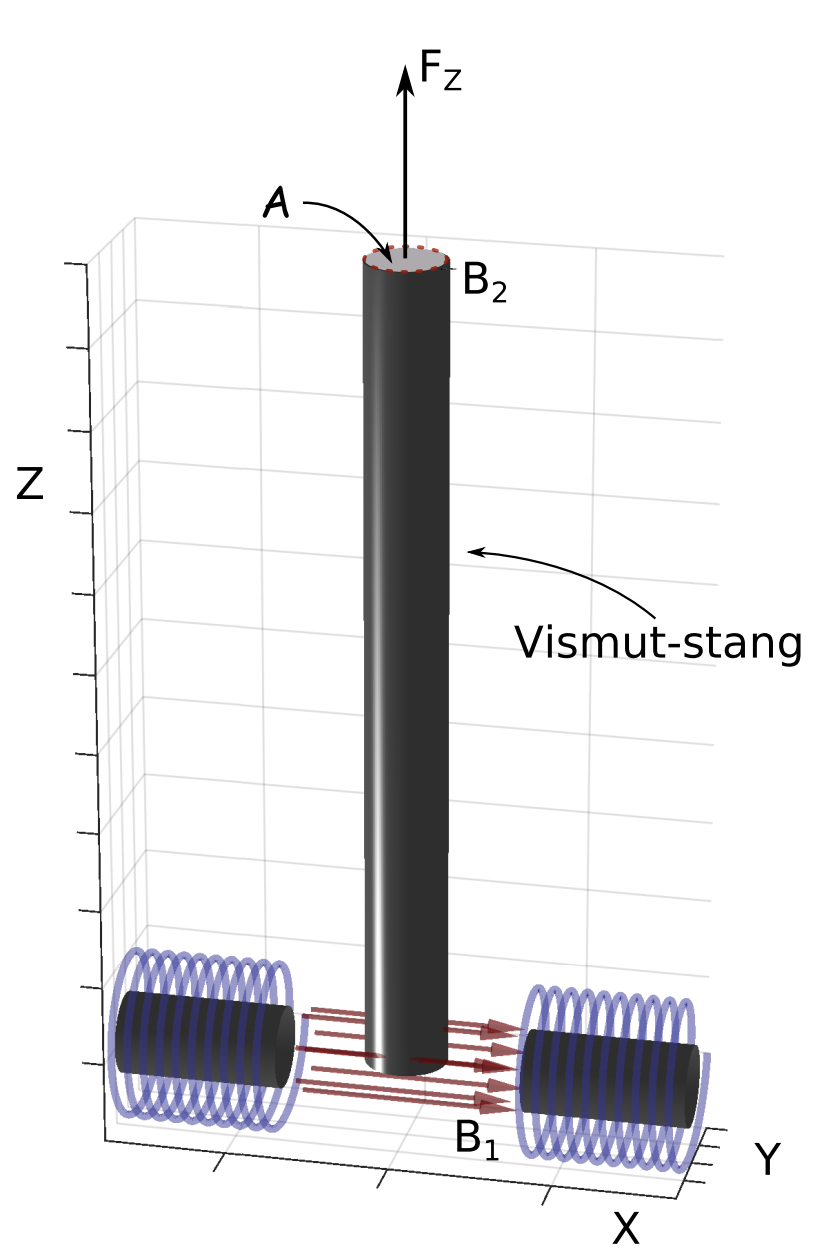
\includegraphics[scale=0.38]{oppsett1.png}
  \caption{Illustrasjon av vismutstang i magnetfelt brukt for å måle magnetisk susceptibilitet i vismut. I figuren ser vi de forskjellige størrelsene som trengs å måle under eksperimentet, $B_1$, $B_2$, $A$ og $F_z$, til å kunne beregne susceptibiliteten. De blå sirklene representerer strømspolen som generer magnetfeltet. Fiugren er hentet fra \cite{oppgave}.}
  \label{eksperimentelt_oppsett1}
\end{figure}
Under eksperimentet varierte vi strømmen i kretsen fra $\SI{0}{\ampere}$ til $\SI{2.4}{\ampere}$, med en lineær økning på $\SI{0.2}{\ampere}$. Størrelsen til den magnetiske kraften som virker på vismut staven er gitt av \eqref{vismut}, som gjør at vi trenger å måle tversnittsarealet, kraften, og magnetfeltet for å kunne beregne susceptibiliteten. Tversnittsarealet beregnes ved å måle diameteren til stangen med et skyvelær. Målingen av diameteren ble gjort på flere punkter langs vismutstangen, itilfellet at tversnittsarealet ikke var konstant. Magnetfeltet måles uten at vismut staven er i magnetfeltet, ved å feste en hall-sonde, og lese av målingen til hall-sonden mens vi varierer strømstyrken. Dette måtte gjøres to ganger, med to forskjellige festinger, for å måle både $B_1$ og $B_2$. \\
Vistmutstangen er festet i et tau, dette tauet festes i en krok. Denne kroken hviler på en presisjonsvekt. På grunn av retningen til magnetfeltet vet vi at retningen på den magnetiske kraften. Fra dette kan vi nullstille vekten, og lese av endringen i vekt som funksjon av strømstykre, som gjør at vi kan beregne $F_z$ som en funksjon av strømstyrken.
\subsection{Ferromagnetisme}
I denne delen av eksperimentet ønsker vi å undersøke de magnetiske egenskapene til jern på to forskjellige måter. Ført ønsker vi å studere jernklumper inn i en spole, og deretter studere hysteresetap til en jernsylinder. \par
Først skal vi gjøre målinger på fire forskjellige jernklumber med ulik geometri inne i en stor spole, som generer et tilnærmet homogent magnetfelt på innsiden. Spolen har $244$ vindinger, og en lengde på $\SI{275}{\milli\meter}$. Jernklumpene har fire forskjellige geometrier vi ønsker å studere: kule, stang, ellipsodial og skive. En illustrasjon av oppsettet brukt under eksperimentet er vist i figur \vref{eksperimentelt_oppsett2}.
\begin{figure}[h!]
  \centering
  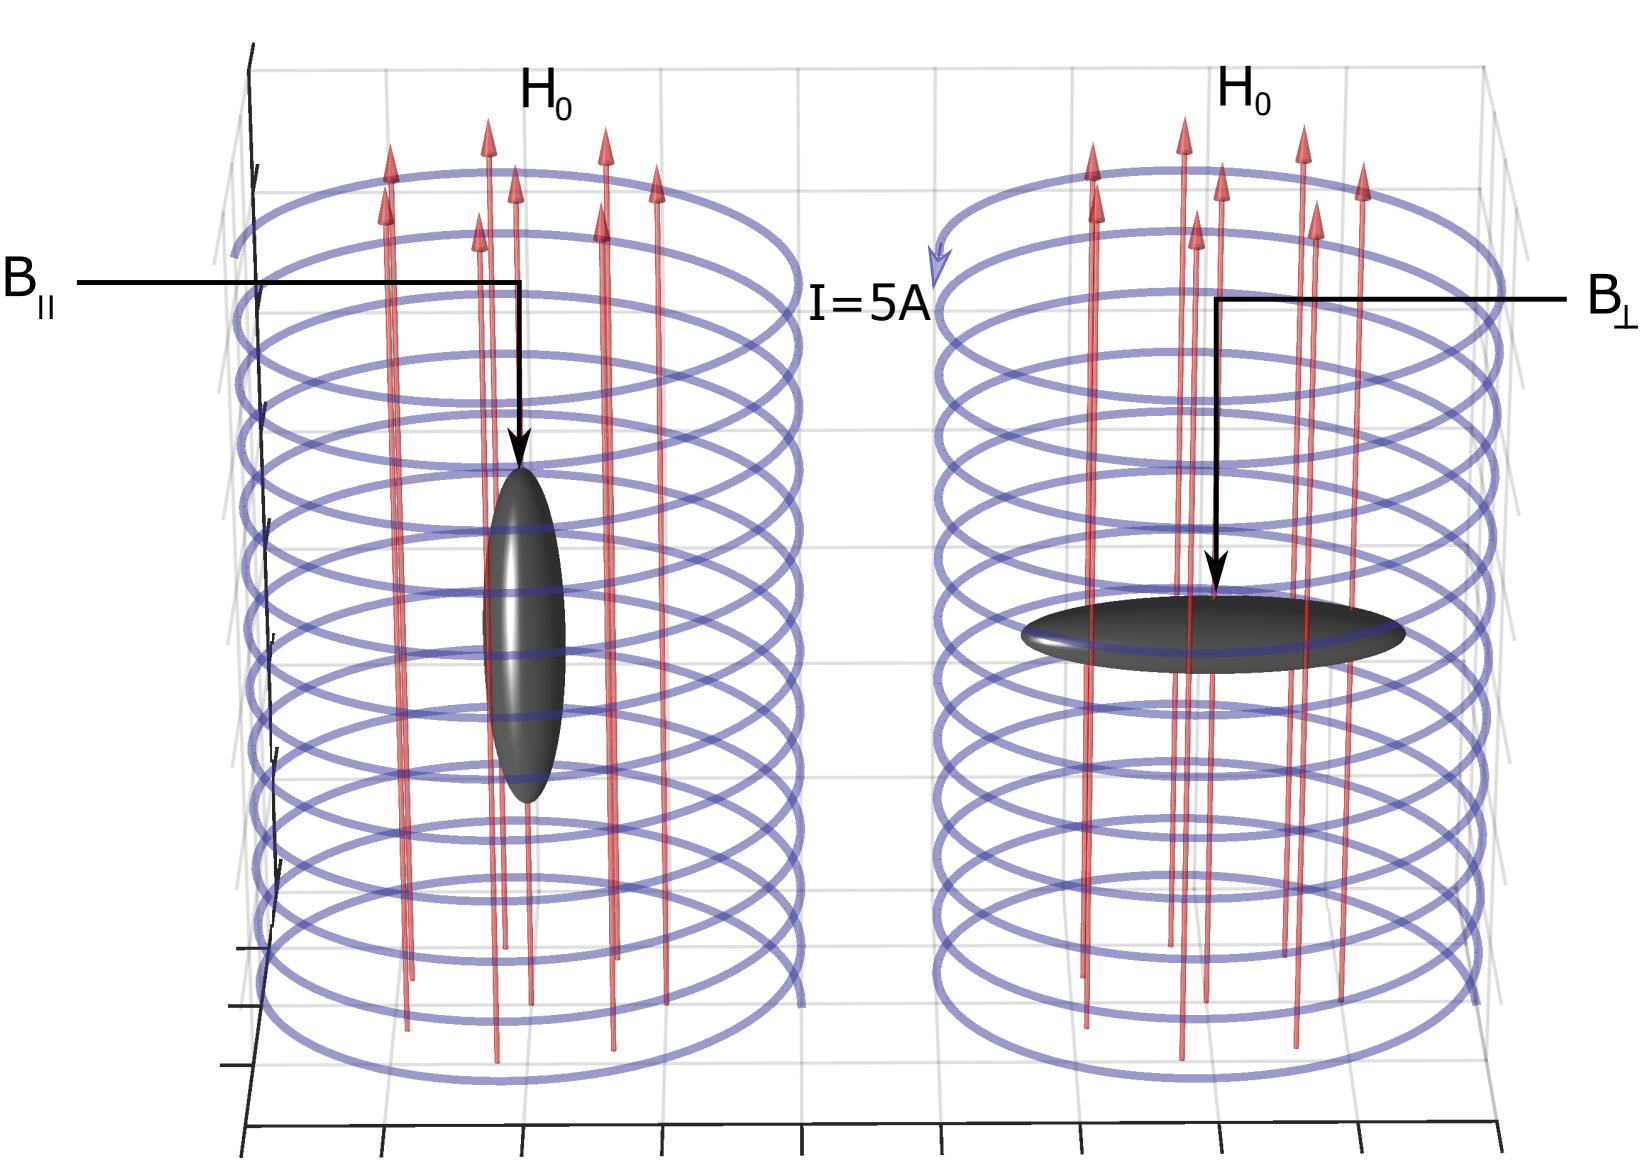
\includegraphics[scale=0.3]{oppsett2.png}
  \caption{Illustrasjon av ellipsodial jernklump inne i en spole. I figuren er det vist med rotasjonsaksen til jernklumpen parallellt med magnetfelt (venstre), og rotasjonsaksen til jernklumpen ortogonalt på magnetfeltet (høyre). De røde linjene viser retningen på magnetfeltet, og de blå linjene viser spolen som jernklumpen blir plassert i. Fiugren er hentet fra \cite{oppgave}.}
  \label{eksperimentelt_oppsett2}
\end{figure}
Før vi gjør målinger med jernklumpene inne i spolen måler vi magnetfeltet inne i spolen, når det går en strøm på $\SI{5}{\ampere}$, forskjellige steder i spolen. Dette blir gjort ved hjelp av en hall-sonde. Under målingene passer vi på at hallsonden står normalt på magnetfeltet, for å få mest presise målinger.\\For å ha jernklumpene i sentrum av spolen blir det brukt plastikkstativ som plaseres inne i spolen. Vi gjentar derfor målingene av magnetfeltet med hall-sonden, men nå med plastikkstativet for å teste om dette påvirker magnetfeltet inne i spolen. For å vite eksentrisiteten til de fire geometriske formene gjorde vi målinger av lengden til objektene langs, og på tvers av, rotasjonsaksene, med skyvelær. Fra disse verdiene kunne vi beregne eksentrisiteten ved \eqref{eksent}.\\
Deretter ble det gjennomført målinger av magnetfeltet på overflaten til hver av de fire jernklumpene, mens de var plassert i spolen, med strømmen til spolen på. Målingene ble gjort for hver av klumpene med rotasjonsaksen parallelt med magnetfeltet, og rotasjonsaksen ortogonalt på magnetfeltet. På grunn av lengden til ellipsoiden fikk den ikke plass med rotasjonsaksen ortogonalt på magnetfeltet.\par
Vi ønsker nå å se på de magnetiske egenskapene til jern ved å studere hysteresekurver. For å gjøre dette plasserer bruker vi en lang jernstang med en spole, sekundærspolen, tvunnet rundt seg. Jernstangen, med sekundærspolen rundt, skal plasseres inne i primærspolen. Primærspolen er koblet til en spenningsgenerator. Spenningsintegratoren gir oss integralet av forskjellen i elektrisk potensial, mellom endepunktene av sekundærspolen, som er gitt av \eqref{deltas}. Faraday's induksjonslov \eqref{2}, gir oss en kobling mellom spenningsforskjellen over en strømsløyfe, og endringen av den magnetiske flukstetthet over tid. Måleapparatet og spenningsgeneratoren er koblet til en dataakvisasjonsboks, som gjør at vi får målingene for styrken til spenningsgeneratoren $S$ som en funksjon av strømmen $I$, direkte inn på datamaskinen. Fra datamaskinen kan vi da beregne verdien for $\Delta S$, og ved likning \eqref{deltab}, beregne endringen i den magnetiske flukstettheten. For å gjøre dette trenger vi å vite antall vinninger, tversnittsarealet til sekundærspolen, og kalibreringskonstanten. All denne informasjonen vet vi fra labratorieutstyret. Under eksperimentet studerer vi hysteresekurvene på datamaskinen, mens vi endrer strømstyrken i primærspolen fra $\SI{0}{\ampere}$ til $\SI{2.4}{\ampere}$, med en lineær økning på $\SI{0.2}{\ampere}$.
\subsection{Faraday effekten}
Faraday effekten viser at lys og magnetiske er knyttet til hverandre. I denne delen av eksperimentet ser vi på effekten magnetfelt har på lys med tre forsjellige bølgelengder, $\lambda = 440, 580, \SI{595}{\nano\meter}$. Et figur av det eksperimentelle oppsettet er vist i figur \vref{eksperimentelt_oppsett3}.
\begin{figure}[h!]
  \centering
  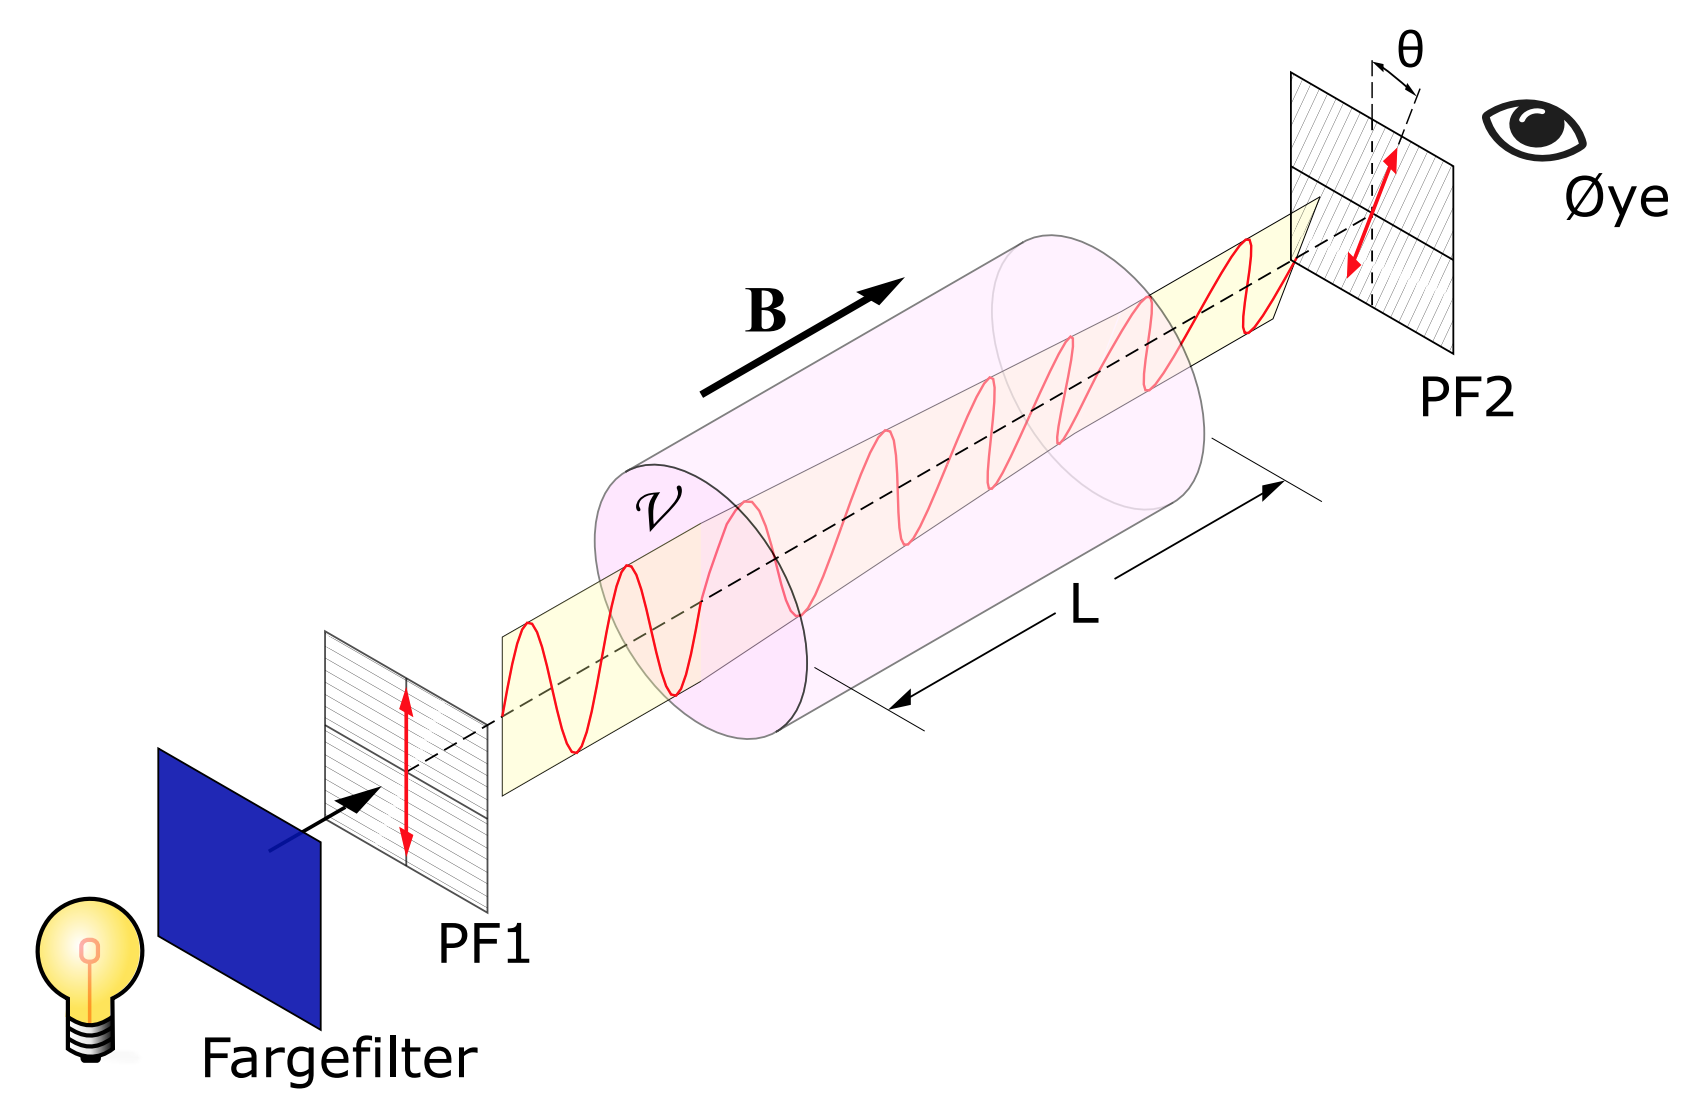
\includegraphics[scale=0.3]{oppsett3.png}
  \caption{Illustrasjon av eksperimentelt oppsett for å måle Faraday effekten. Fra venstre til høyre i figuren ser vi lyskilden som sender lys gjennom et fargegitter, som bare slipper gjennom øsnkede farger. De monokromatiske bølgene som passerer gjennom fargefilteret går gjennom det første polarisasjonsfilteret, PF1. Det polariserte lyset beveger seg inn i flintglasset med lengde $L$, hvor det er et ytre magnetfelt i bevegelsesretningen til lyset. Før lyset treffer øyet må det passere gjennom det andre polarisasjonsfilteret, PF2. Ved å endre på dreiningsvinkelen $\theta$ vil en måle polarisasjonen til lyset ved å lete etter dreiningsvinkler som filtrer alt lyset.
  Fiugren er hentet fra \cite{oppgave}.}
  \label{eksperimentelt_oppsett3}
\end{figure}
Får å måle Faraday-effekten gjør vi ved å brukke optiske filtere, som bare slipper gjennom noen ønskede bølgelengder, dette gjør lyset tilnærmet monokromatisk. Videre trenger vi to polarisasjonsfiltere, som plasseres på hver sin side av flintglasset. Når de to polarisasjonsfilterene står $90\degree$ på hverandre, og det ikke er noe magnetfelt, skal en ikke kunne se noe lys gjennom polarisasjonsfilterene. Ved å endre på styrken på magnetfeltet, ved å endre på strømmen som induserer et magnetfelt, ønsker vi å finne hvilken dreiningsvinkel til polarisasjonsfilteret som filtrer alt lyset. Målingene blir gjort med magnetfeltet peke i begge retninger. Fra å finne forholdet mellom dreiningsvinkelen $\theta$ og styrken på magnetfeltet $B$, samt vite lengden av flintglasset $L$ kan vi beregne verdet konstanten fra likning \eqref{verdet}.
I eksperimentet økte vi strømstyrken med $\SI{0.5}{\ampere}$ fra $\SI{0}{\ampere}$ til $\SI{3.0}{\ampere}$, i både positiv og negativ strømretning. Styrken på magnetfeltet inne i flintglasset er en faktor $1.5$ mindre enn styrken på magnetfeltet målt midt mellom polene.
\section{\label{sec:level4}Resultater}
\subsection{Diamagnetisme}
Ved å måle diameteren til vismut prøven på fire forskjellige punkter måle vi $\SI{10.03}{\milli\meter}$ to steder, og $\SI{10.06}{\milli\meter}$. Ved å ta hensyn til spredningen i disse målingene, og usikkerheten til skyvelæret brukt, finner vi at diameteren til vismut prøven er $\SI{10.05\pm0.03}{\milli\meter}$. Dette resulterer i at tversnittet til vismutprøven er $\SI{79.3\pm0.2}{\milli\meter^2}$.\\
Halvparten av målingene for strøm $I$, magnetfelt mellom spolene $B_1$, magnetfelt ved toppen av vismutprøven $B_2$, og kraften på vekten $F_z$, er vist i tabell \vref{table_vismut}.
\begin{table}
  \centering
  \caption{Målinger av strøm $I$, magnetfelt mellom spolene $B_1$, magnetfelt ved toppen av vismutprøven $B_2$, og kraften på vekten $F_z$, for å beregne den magnetiske susceptibiliteten til vismutprøve. Halvparten av målingene er vist i tabellen. Usikkerhetene i tabellen kommer henholdsvis fra databladet til strømgeneratoren, spredning og oppløsning til hallsonden, spredning og oppløsning til hallsonden, og databladet til vekten.}
  \label{table_vismut}
    \begin{tabular}{@{}llll@{}}\botrule
    $I$ {[}A{]} & $B_1$ {[}mT{]} & $B_2$ {[}mT{]} & $F_z$ {[}mN{]} \\ \colrule

    0.000(3)    & 18.0(3)        & 0.4(1)         & 0.00(10)      \\
    0.400(7)    & 185(2)         & 1.2(1)         & 0.02(10)      \\
    0.80(1)     & 356(4)         & 2.0(1)         & 0.06(10)      \\
    1.20(2)     & 505(5)         & 2.3(1)         & 1.3(1)        \\
    1.60(2)     & 628(6)         & 2.4(1)         & 2.0(1)        \\
    2.00(5)     & 719(7)         & 2.5(1)         & 2.6(1)        \\
    2.40(5)     & 788(8)         & 2.3(1)         & 3.0(1)        \\\botrule
    \end{tabular}
\end{table}
Målingene av den magnetiske suceptibiliteten som funksjon av magnetfeltet mellom spolene er vist i figur \vref{resultat_chi}.
\begin{figure}[h!]
  \centering
  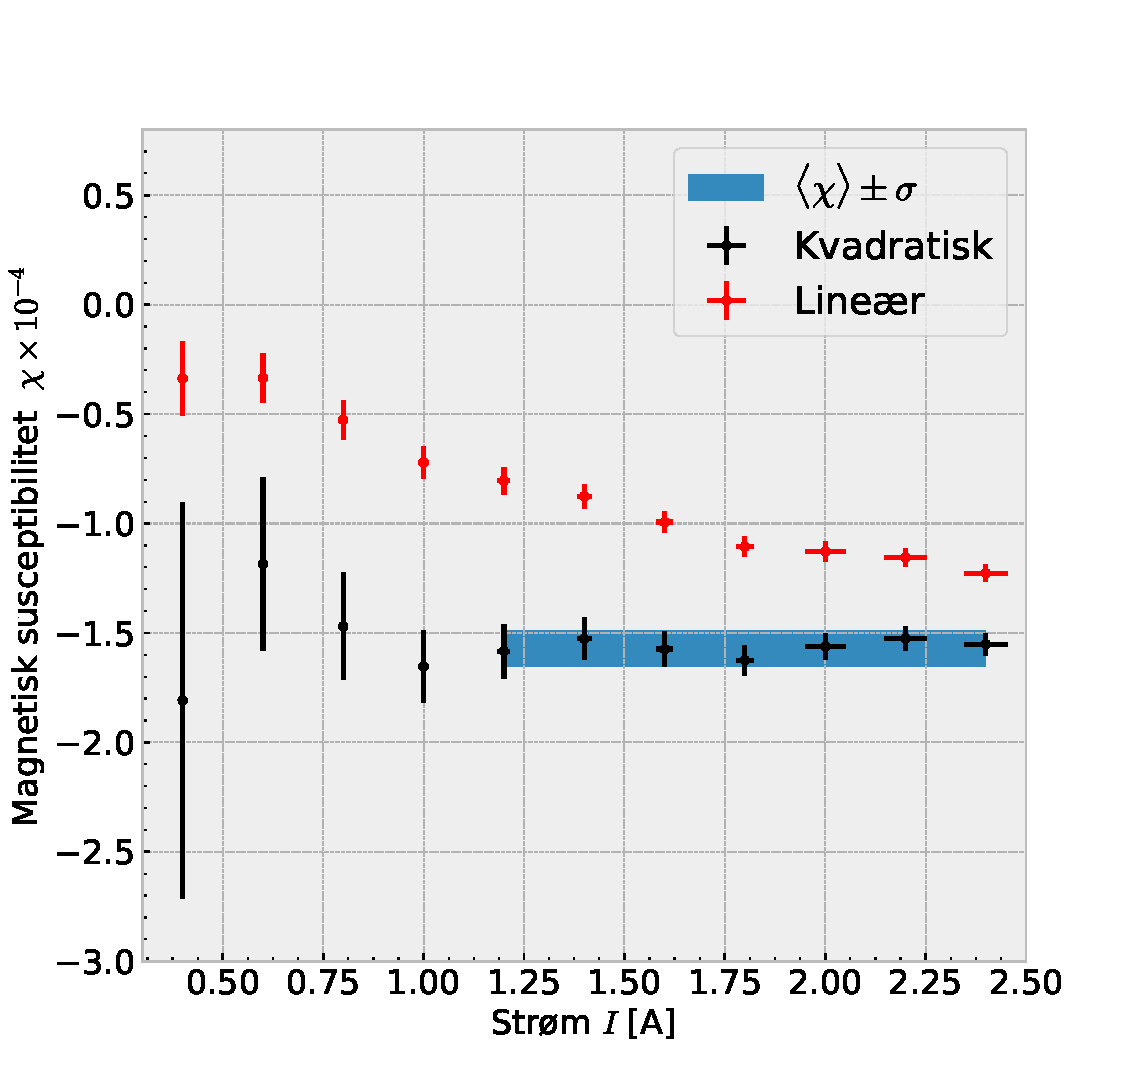
\includegraphics[scale=0.4]{chi_effekt.pdf}
  \caption{Den magnetiske susceptibiliteten $\chi$ som funksjon av magnetfeltet $B_1$ mellom spolene. Det blå området i grafen viser gjennomsnittet, og spredningen i gjennomsnittet til de siste målepunktene. Den gjennomsnittlige verdien for de $8$ siste målepunktene er $\chi = -1.57(4)$.}
  \label{resultat_chi}
\end{figure}
\subsection{Ferromagnetisme}
Vi ønsker nå å studere de magnetiske egenskapene til jern med ved å måle styrken på magnetfeltet, mens jernklumpen er plasert i en spole. For å sammenlikne resultatene med teori trenger vi de geometriske størrelsene til de fire jernklumpene vi skal se på. Det ble derfor gjennomført målinger av diameter og høyde med et skyvelær, resultatene er vist  i tabell \vref{tot_ferro}.
Ved å sende en strøm på $\SI{5}{\ampere}$ i sløyen generes det et magnetfelt inne i spolen. Vi bruker en hallsonde til å måle styrken på magnetfeltet, over flere målinger finner vi at styrken på magnetfeltet er $\SI{5.04\pm0.04}{\milli\tesla}$, usikkerheten kommer fra spredningen i målingene. \\
Deretter ble det målt styrken på magnetfeltet med plastikkstativet inne i spolen. Endringen i styrken på magnetfeltet var innenfor usikkerheten til magnetfeltet. Plastikkstativet påvirker altså ikke magnetfeltet inne i spolen. \\
De fire jernklumpene ble plassert på plastikkstativet, inne i spolen, med strømmen på. Ved å måle styrken på magnetfeltet på overflaten til jernklumpen med en hallsonden rettet parallellt med feltet, fikk vi målingene vist i tabell \vref{tot_ferro}.\par
\begin{table*}\renewcommand{\arraystretch}{1.2}
\centering
\caption{I denne tabellen er det vist de geometriske størrelsene til jernklumpene, parallellt med rotasjonsakse ($a_{\parallel}$) og tangensialt på rotasjonsaksen ($a_{\perp}$). Fra disse måline kan en beregne avmagnetiseringsfaktoren parallellt med magnetfeltet ($D_{\parallel}$) og tangensialt på magnetfeltet ($D_{\perp}$). Usikkerheten til målingene kommer fra usikkerheten til skyvelæret, og usikkerhetn til avmagnetiseringsfaktoren kommer av \eqref{usikkerhet1}. Videre i tabellen vises styrken til magnetfeltet i kontakt med jernklumpen, når rotasjonsaksen til jernklumpen er parallell med magnetfeltet ($B\parallell$) og tangensialt på magnetfeltet ($B\perp$). Usikkerheten er beregnet fra databladet til hallsonden. For å teste teorien \eqref{ikke_enda} inkluderer tabellen $B_0/D_i$, som indikerer øvre grense for $B_i$, hvor $i$ enten indikerer parallell $\parallel$ eller ortogonalt $\perp$.}
\label{tot_ferro}
\begin{tabular}{@{}lllllllll@{}}
\botrule
Form & $a_{\parallel}$ {[}cm{]} $\quad$  & $a_{\perp}$ {[}cm{]} $\quad$  & $D_{\parallel}$ $\qquad \quad$ & $D_{\perp}$ $\qquad\quad$ &  $\bm{B}$  $\parallel$ {[}mT{]} $\quad$ & $\bm{B}$ $\perp$ {[}mT{]} $\quad$ & $B_0/D_{\parallel}$ [mT]$\quad$  & $B_0/D_{\perp}$ [mT]\\ \colrule

Skive      & 0.67(1)        & 5.99(2)           & 0.99(8)         & 0.005(4) & 5.50(1)                           & 17.58(4)         &    5.1(4)  &  1036(86)      \\
Ellipsoide & 21.8(2)        & 0.96(1)           & 0.055(8)        & 0.50(5) & 50.5(1)                           & -                &   920(80)    & 10.1(8)       \\
Sylinder   & 6.45(2)        & 0.98(1)           & 0.037(3)        & 0.48(4) & 19.65(4)                          & 7.74(2)          &   133(11)    &10.5(9)           \\
Kule       & 6.32(2)        & 6.32(2)           & 0.33(3)         & 0.33(3) & 12.61(3)            & 12.61(3)                &   15(1)  & 15(1)        \\ \botrule
\end{tabular}
\end{table*}
Vi kan også studere magnetfeltet rundt en jernklump ved å se på hysteresekurver. Under eksperimentet ble det brukt en sekundærspole med $n=135$ vindinger, og en diameteren til sekundærspolen var $\SI{6.5pm0.1}{\milli\meter}$, som gjør at arealet er $\SI{33\pm1}{\milli\meter^2}$. Kalibreringskonstanten $\kappa$ til spenningsgeneratoren var oppgit til å være $\SI{1.01}{\micro\weber}$. Fra disse verdiene kan vi beregne endringen i magnetfelt fra likning \eqref{deltas}, det eneste som mangler er $\Delta S$. Integralet fra spennignsgeneratoren $\Delta S$ ble vist gjennom koblingen til data dataakvisasjonsboksen, som gjorde at vi fikk direkte målinger av integralet til spenningsgeneratoren. Det eneste som trenkte å endres var styrken på strømmen $I$. Resultatene er vist grafisk i figur VREF. Et eksempel på målinger fra dataakvisasjonsboksen er vist i figur VREF.
\subsection{Faraday-effekten}
For å beregne verdet-konstanten ble det gjennomført målinger av polarisasjonsgraden til lys som funksjon av styrken på det ytre magnetfeltet. Disse målingene er vist i tabell \vref{faraday}. Fra å beregne stigningstallet til polarisasjonsvinkelen som funksjon av produktet mellom magnetfeltet og lengden på flintglasset \eqref{verdet} kunne vi beregne verdet-konstanten. Verdien til verdetkonstanten er vist for de tre forskjellige bølgelengdene er vist i tabellen.
\begin{table}\renewcommand{\arraystretch}{1.1}
  \centering
  \caption{I denne tabellen er det vist målt vinkel for $\theta [\degree]$, for forskjellig styrke i magnetfelt, og forskjellig strømretning. Usikkerheten i vinkelen er lik $0.2\degree$ for alle målinger, siden dette var oppløsningen til måleapparatet. Nederest i tabellen er det beregnet stigningstall for målepunktene i både negativ og positiv strømretning for hver bølgelengde. Usikkerheten i stigningstallet kommer fra lineærregresjonen.}
  \label{faraday}
  \begin{tabular}{|l|S|S|S|S|S|S|}
    \colrule
      Bølgelengde $\lambda$ [nm] &
      \multicolumn{2}{|c|}{$440$} &
      \multicolumn{2}{c|}{$580$} &
      \multicolumn{2}{c|}{$595$} \\
      \colrule

      $B$ [mT] & \multicolumn{6}{c|}{Vinkel $\theta\pm0.003$ [radianer] } \\   \colrule

      43(1)  & 0.031 & 0.024 & 0.031 & 0.024 & 0.035 & 0.028 \\
      63(1)  & 0.049 & 0.038 & 0.045 & 0.035 & 0.049 & 0.045 \\
      83(2)  & 0.066 & 0.052 & 0.052 & 0.049 & 0.062 & 0.056 \\
      102(2) & 0.073 & 0.070 & 0.070 & 0.059 & 0.077 & 0.073 \\
      119(3) & 0.091 & 0.084 & 0.077 & 0.070 & 0.091 & 0.084 \\ \colrule

      Strømretning & {$I_+$} & {$I_-$} & {$I_+$} & {$I_-$} & {$I_+$} & {$I_-$} \\ \colrule
      Stigningstall [radianer/Tm] &
      \multicolumn{2}{|c}{$26\pm2$} &
      \multicolumn{2}{|c}{$24\pm1$} &
      \multicolumn{2}{|c|}{$20\pm2$} \\
      \colrule
  \end{tabular}
\end{table}
Et sett av målinger er vist i figur \vref{fig_verdet}. Figuren viser polarisasjonsvinkel $\theta$ som funksjon av produktet mellom magnetfelt og lengden på flintkrystallen. For målingene vist i figuren er det brukt lys med bølgelengde $\lambda=\SI{580}{\nano\meter}$. Det skraverte området i figuren viser usikkerheten i stigningstallet, og den stiplede linjen viser gjennomsnittet til stigningstallet, som blir verdien for verdet konstanten ved denne bølgelengden.
\begin{figure}[ht!]
  \centering
  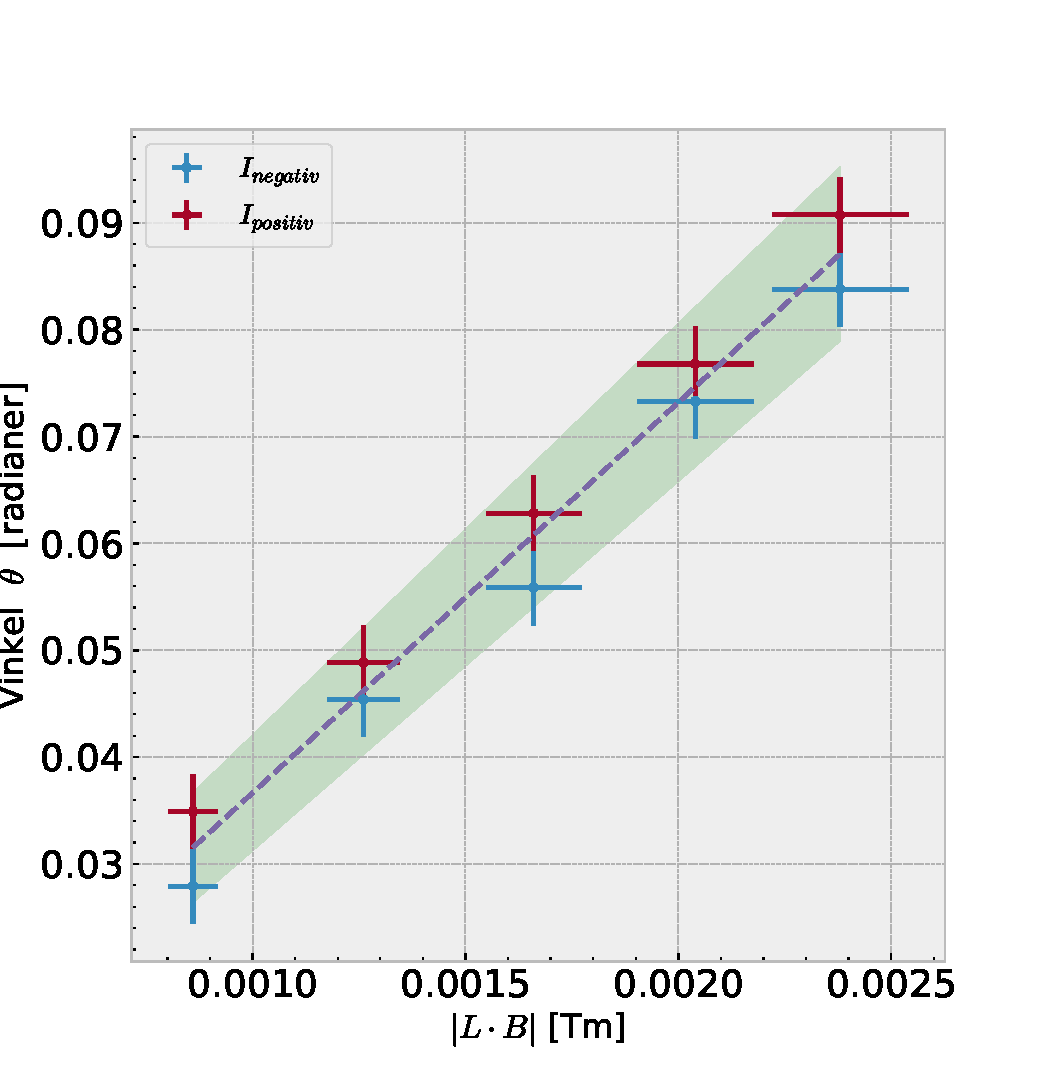
\includegraphics[scale=0.38]{faraday_effekt.pdf}
  \caption{Målinger for polarisasjonsvinkel $\theta$ som funksjon av absolutverdien til produktet mellom styrken til magnetfeltet og lengden av flintkrystallen, for bølgelengde på $\lambda=\SI{580}{\nano\meter}$. Fra målepunktene beregnes det stigningstallet ved hjelp av lineærregresjon, som er verdet-konstanten. For denne bølgelengden var verdetkonstanten $1.4\pm0.1$k/Tm}
  \label{eksperimentelt_oppsett1}
\end{figure}
\section{Diskusjon}
\subsection{Diamagnetisme}
Verdiene brukt for å beregne den magnetiske suceptibiliteten er vist i figur \vref{resultat_chi}. Som vi ser i figuren avtar usikkerhetn som styrken på strømmen øker. Dette er fordi den relative usikkerheten til vekten er stor når utslaget på vekten er lite. For å beregne verdien til $\chi$ bruker vi derfor en vektet midlig på de $8$ siste punktene. Målingene med høyere usikkerhet blir vektet lavere i beregningen av gjennomsnittet til de siste $8$ målingene. Dette resultert i at verdien til den magnetiske suceptibiliteten blie $\chi =$.
I tabell \vref{table_vismut} er målingene gjort for å beregne den magnetiske suceptibiliteten vist. Fra verdiene ser vi at kraften som virker på vismutstangen øker med styrken på magnetfeltet. Som strømmen i spolene øker, øker kraften på den magnetiske flukstettheten. Den magnetiske flukstettheten mellom spolene $B_1$ øker nesten lineært med strømstyrken, men mot slutten avtar stigningen svakt. Styrken på magnetfeltet på den andre enden av staven går mot en konstant verdi på rundt $\SI{2.4}{\milli\tesla}$, når strømmen når $\SI{1.20}{\ampere}$. Fra å bruke likning \eqref{test_chi} kan vi teste effekten av å sette $B_2=\SI{0}{\tesla}$. Verdien til $\chi$ blir mer nøyaktig, jo sterke magnetfeltet er, vi bruker derfor verdien til den magnetiske flukstettheten for strømmen $I=\SI{2.4}{\ampere}$. Dette gir oss en endring av $\chi$ på SETT INN VERDI HER. Altså har det tilnærmet ingen effekt ved å inkludere $B_2$ i beregningen av suceptibiliteten. Faktisk vil økningen av usikkerheten øke med $...$ ved å inkludere $B_2$, som er større enn endringen i suceptibiliteten. Det vil derfor gi mer presise resultater ved å ikke inkludere $B_2$, enn å gjøre det, selv om dette er nærmere det analytiske uttrykket.
\subsection{Ferromagnetisme}
Målingene gjort for de fire forskjellige jernklumpene er vist i tabell \vref{tot_ferro}. Denne tabellen inkluderer målingene av lengden til de fire jernklumpene, parallellt med, og tangensialt på, symetriaksen.
Fra tabellen ser vi at lengden til ellipsoiden parallellt med symmetriaksen har en mye større usikkerhet enn de andre lengdene. Årsaken til dette er at dette målet måtte bli gjort med en meterstokk istedenfor et skyvelær, som gir oss en mye større usikkerhet. Denne usikkerheten manififisterer seg ikke merkbart i de følgende usikkerheten for ellipsoiden. Fra lengden til jernklumpene kunne vi beregne avmagnetiseringsfaktoren til jerklumpen parallelt med, og ortogonalt på rotasjonsaksen. Disse brukes til å finne den øvre grensen for magnetfeltet når symetriaksen til jerklumpen er plassert henholdsvis parallellt med og ortogonalt på magnetfeltet ved likning \eqref{}.
%\begin{thebibliography}{9}
%\bibitem{squires}
%Squires, G.L. \emph{Practical Physics}, Cambridge University Press, 2001.
%\bibitem{oppgave}
%Univseritet i Oslo \emph{Magnetisme}, 2018
%\end{thebibliography}
\bibliography{citations.bib}{}
\bibliographystyle{plain}
\end{document}
